% AstroAgentBench — AACL-IJCNLP 2026 presentation slides (16:9)
% Build: latexmk -pdf -interaction=nonstopmode -halt-on-error -outdir=build slides.tex
\documentclass[aspectratio=169,11pt]{beamer}

\usetheme{moloch}
\molochset{sectionpage=none}
\usepackage[T1]{fontenc}
\usepackage[utf8]{inputenc}
\usepackage{graphicx}
\usepackage{booktabs}
\usepackage{colortbl}
\usepackage{tabularx}
\usepackage{tikz}
\usetikzlibrary{positioning,arrows.meta}

% ---- brand ----
\definecolor{abnavy}{HTML}{102C51}
\definecolor{abcyan}{HTML}{0096BF}
\definecolor{ablight}{HTML}{EAF3F8}
\definecolor{abgray}{HTML}{5A6B7C}
\definecolor{abgold}{HTML}{B8862D}
\definecolor{abred}{HTML}{B03A2E}
\definecolor{abgreen}{HTML}{1E8449}

\setbeamercolor{normal text}{fg=abnavy,bg=white}
\setbeamercolor{frametitle}{bg=abnavy,fg=white}
\setbeamercolor{title separator}{fg=abcyan}
\setbeamercolor{progress bar}{fg=abcyan}
\setbeamercolor{alerted text}{fg=abred}
\setbeamercolor{block body}{bg=ablight,fg=abnavy}

\newcommand{\srcnote}[1]{{\tiny\color{abgray}#1\par}}
\newcommand{\cardtitle}[2][abnavy]{{\small\bfseries\color{#1}#2\par}\vspace{0.15em}}
\newcommand{\stat}[3][abcyan]{{\centering{\huge\bfseries\color{#1}#2\par}\vspace{0.1em}{\scriptsize\color{abgray}#3\par}}}

\hypersetup{
  pdftitle={AstroAgentBench: Evaluating Agentic Planning on Space Mission Planning Tasks},
  pdfauthor={Weiyi Wang, Xinchi Chen, Jingjing Gong, Xuanjing Huang, Xipeng Qiu}
}

\graphicspath{{../assets/}}

\title{AstroAgentBench: Evaluating Agentic Planning on Space Mission Planning Tasks}
\author{Weiyi Wang \and Xinchi Chen\textsuperscript{\dag} \and Jingjing Gong \and Xuanjing Huang \and Xipeng Qiu\textsuperscript{\dag}}
\institute{Fudan University \,\textperiodcentered\, Shanghai Innovation Institute \,\textperiodcentered\, OpenMOSS Team\quad \textsuperscript{\dag}\,Corresponding authors}
\date{AACL-IJCNLP 2026}

\begin{document}

% ================= 1. Title =================
\begin{frame}[plain]
  \begin{tikzpicture}[remember picture, overlay]
    \node[anchor=north, yshift=-1.4em] at (current page.north)
      {
\includegraphics[height=0.95cm]{logo.pdf}};
  \end{tikzpicture}
  \titlepage
\end{frame}

\section{Motivation}

% ================= 2. Hook =================
\begin{frame}{How should these satellites spend the next 12 hours?}
  \begin{columns}[c]
    \column{0.55\textwidth}
      \centering
      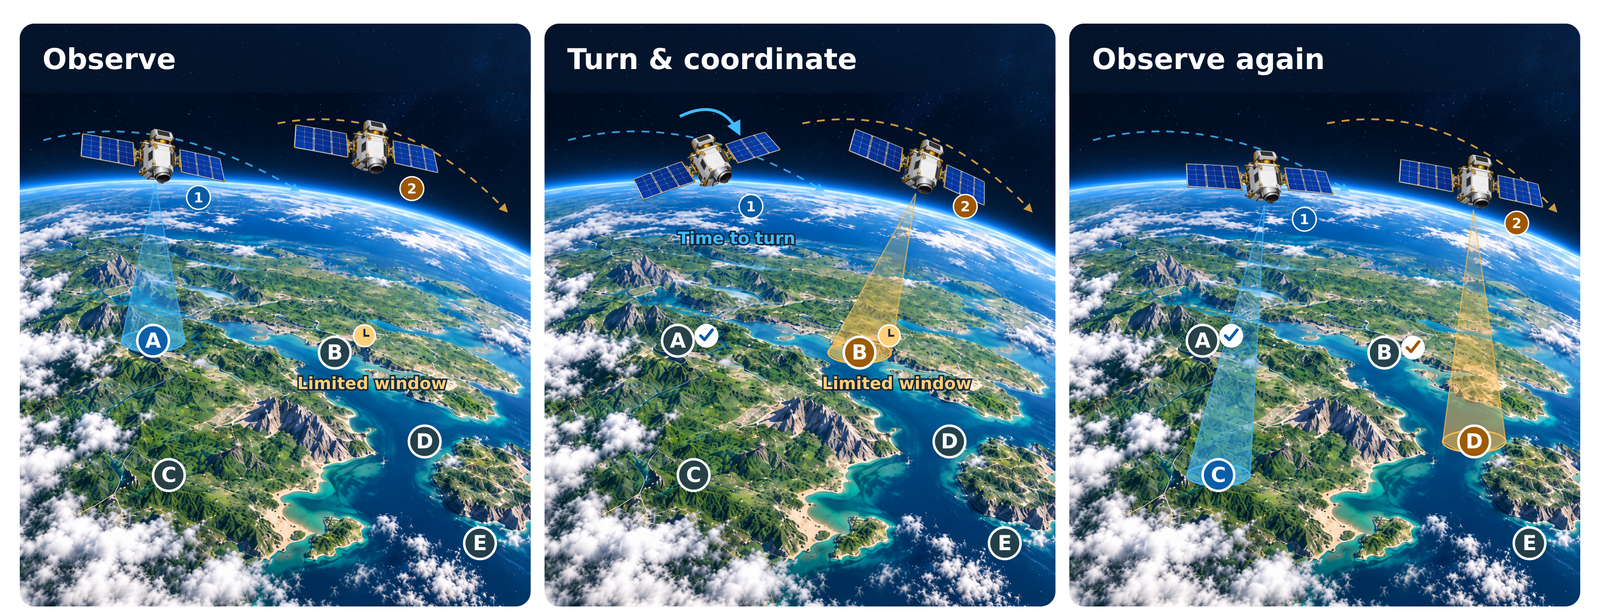
\includegraphics[width=\linewidth]{mission-planning-panels.png}
      \par\vspace{0.3em}
      \srcnote{An illustrative Earth-observation mission. Geometry and timing are schematic.}
    \column{0.43\textwidth}
      {\small
      \begin{itemize}\setlength{\itemsep}{0.55em}
        \item Each target is visible for only \textbf{a few minutes per orbit}, and every slew costs time and power.
        \item Energy and memory form \textbf{one shared budget} across all twelve hours.
        \item A fluent plan can still \textbf{fail in orbit}, arriving after a window closes or draining the battery early.
        \item Once \textbf{uplinked}, the plan cannot be revised, so it must be verified against orbital mechanics in advance.
      \end{itemize}}
  \end{columns}
\end{frame}

% ================= 3. Why a new benchmark =================
\begin{frame}{Executable mission planning needs a verifiable benchmark}
  \small
  \setlength{\tabcolsep}{10pt}
  \begin{tabularx}{\textwidth}{@{}X X@{}}
    {\small\bfseries\color{abnavy}The evaluation gap} & {\small\bfseries\color{abnavy}Three questions}\\[0.45em]
    \textcolor{abgray}{\textbf{G1}}\quad LLM-for-Space evaluations remain \textbf{fragmented} across task formulations, simulators, and success criteria. &
    \textcolor{abcyan}{\textbf{Q1}}\quad Can agents produce plans that \textbf{pass external feasibility checks}, rather than merely describe plausible strategies?\\[0.55em]
    \textcolor{abgray}{\textbf{G2}}\quad A fluent artifact is rarely checked against a \textbf{physically grounded, deterministic verifier}. &
    \textcolor{abcyan}{\textbf{Q2}}\quad When a submission is valid, how close is its \textbf{quality} to that of specialized solver references?\\[0.55em]
    \textcolor{abgray}{\textbf{G3}}\quad A plan can satisfy a schema and still \textbf{observe nothing of value}, so validity alone is too weak. &
    \textcolor{abcyan}{\textbf{Q3}}\quad Which \textbf{system conditions} (verifier use, domain guidance, accumulated experience) explain the variation?\\
  \end{tabularx}
  \vfill
  \centering
  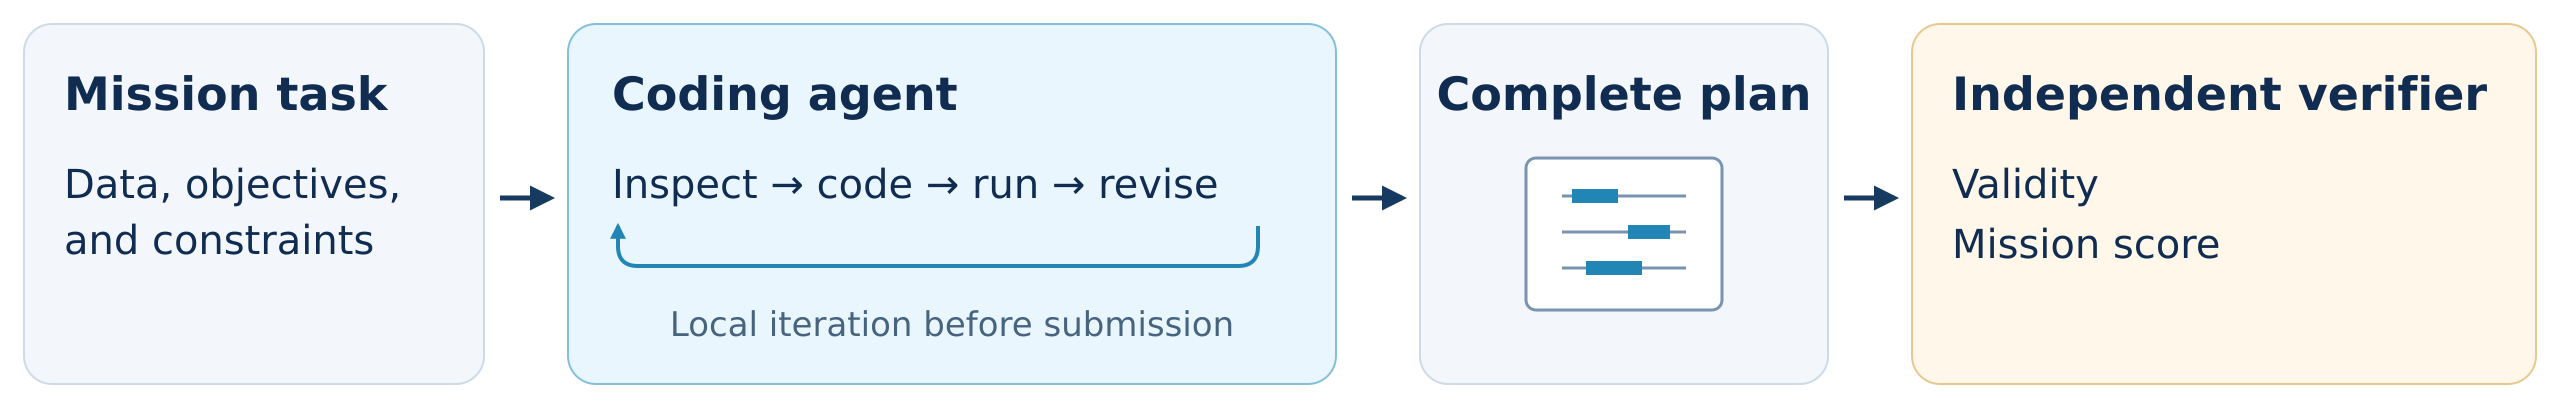
\includegraphics[width=0.98\textwidth]{agent-workflow.png}
\end{frame}

\section{Benchmark}

% ================= 4. Benchmark overview =================
\begin{frame}{Case in, executable plan out, verifier decides}
  \centering
  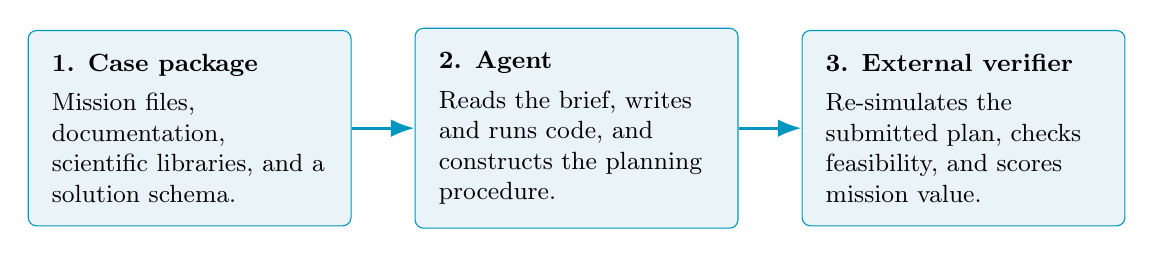
\begin{tikzpicture}[
    stage/.style={rounded corners=3pt, draw=abcyan, fill=ablight, text width=3.5cm, align=flush left, inner sep=0.3cm, font=\small},
    flow/.style={-{Latex[length=3mm]}, line width=1.1pt, draw=abcyan}
  ]
    \node[stage] (case) {\textbf{1. Case package}\\[0.35em] Mission files, documentation, scientific libraries, and a solution schema.};
    \node[stage, right=0.8cm of case] (agent) {\textbf{2. Agent}\\[0.35em] Reads the brief, writes and runs code, and constructs the planning procedure.};
    \node[stage, right=0.8cm of agent] (verifier) {\textbf{3. External verifier}\\[0.35em] Re-simulates the submitted plan, checks feasibility, and scores mission value.};
    \draw[flow] (case) -- (agent);
    \draw[flow] (agent) -- (verifier);
  \end{tikzpicture}
  \par\vspace{1.0em}
  {\small \textbf{116 cases in 7 families}. Each agent \textbf{constructs the planning procedure itself}, writing and running domain code instead of calling a pre-built planner.}
\end{frame}

% ================= 5. Seven families =================
\begin{frame}{Seven families, four kinds of planning decisions}
  \begin{columns}[T]
    \column{0.245\textwidth}\centering
      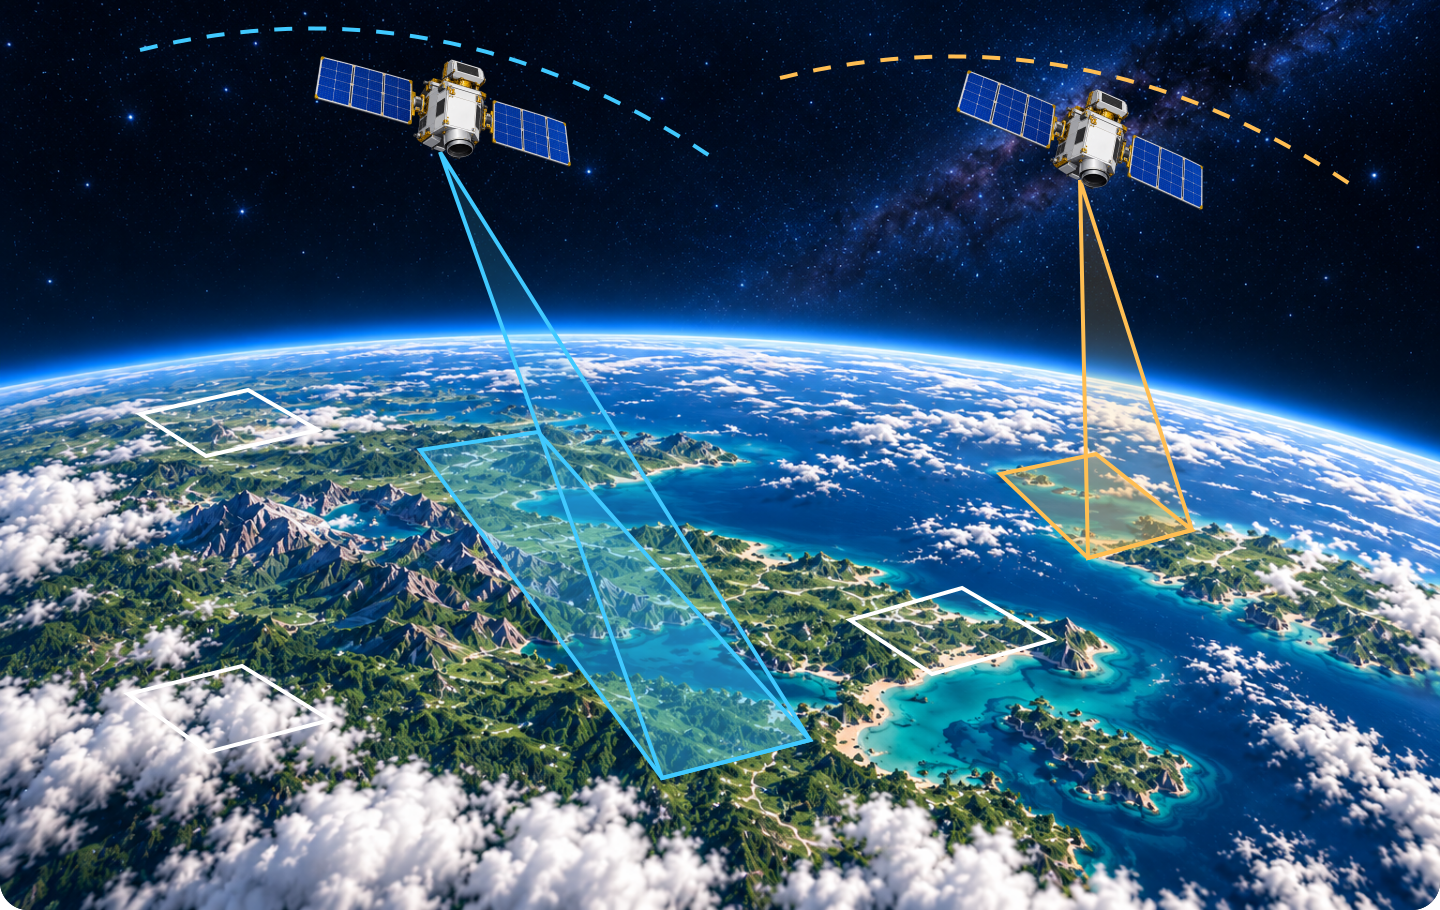
\includegraphics[width=0.94\linewidth]{tour-observe.png}\\[0.08em]
      {\scriptsize\bfseries Observe Earth}\\[0.05em]
      \parbox[t][1.7em][t]{\linewidth}{\centering\tiny AEOSSP \,\textperiodcentered\, SPOT-5}
    \column{0.245\textwidth}\centering
      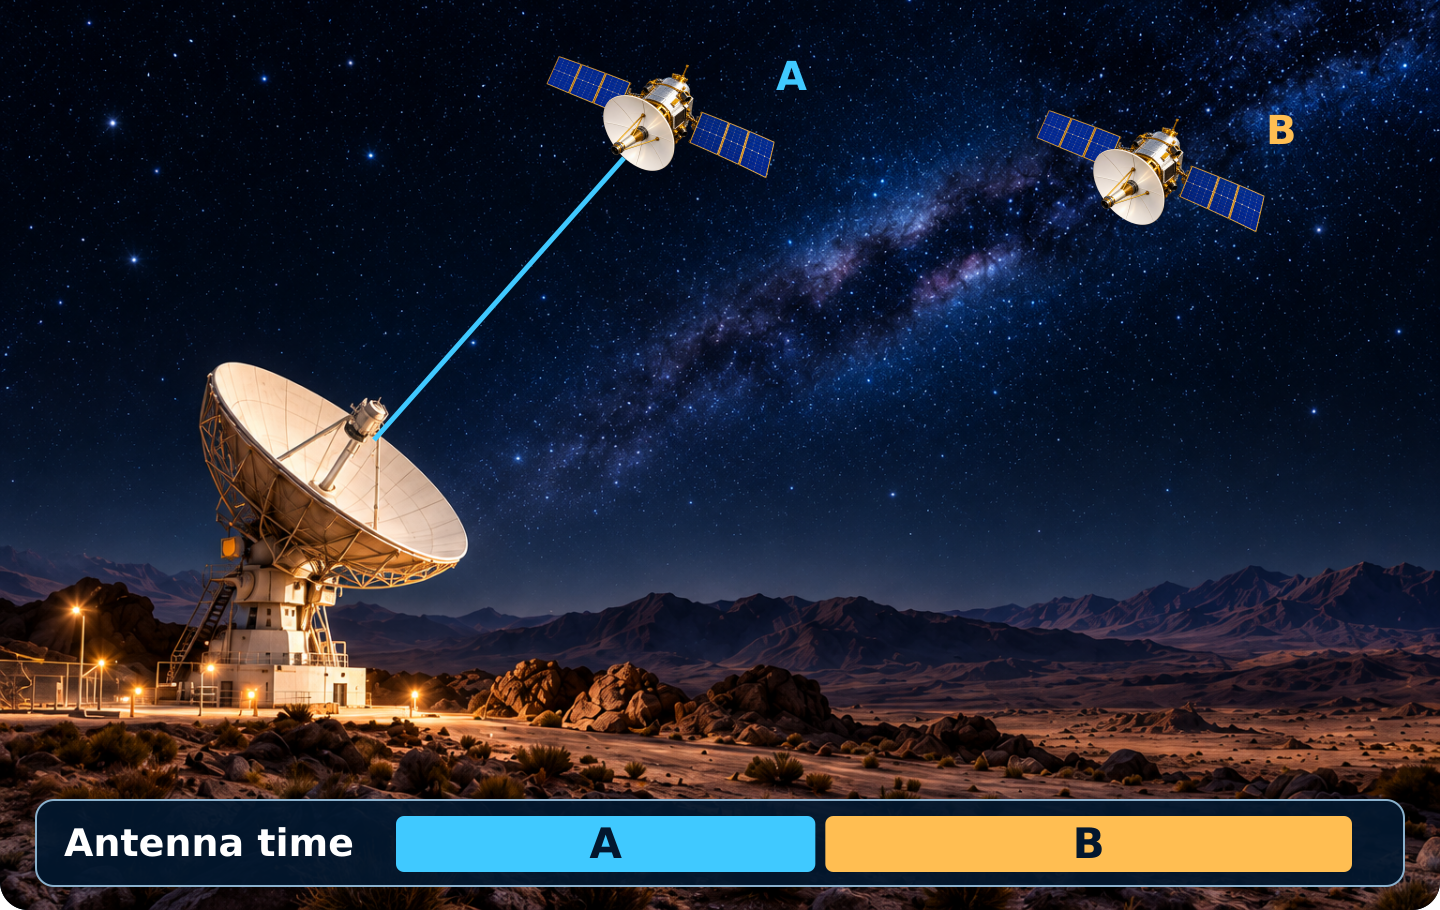
\includegraphics[width=0.94\linewidth]{tour-contacts.png}\\[0.08em]
      {\scriptsize\bfseries Allocate contacts}\\[0.05em]
      \parbox[t][1.7em][t]{\linewidth}{\centering\tiny SatNet}
    \column{0.245\textwidth}\centering
      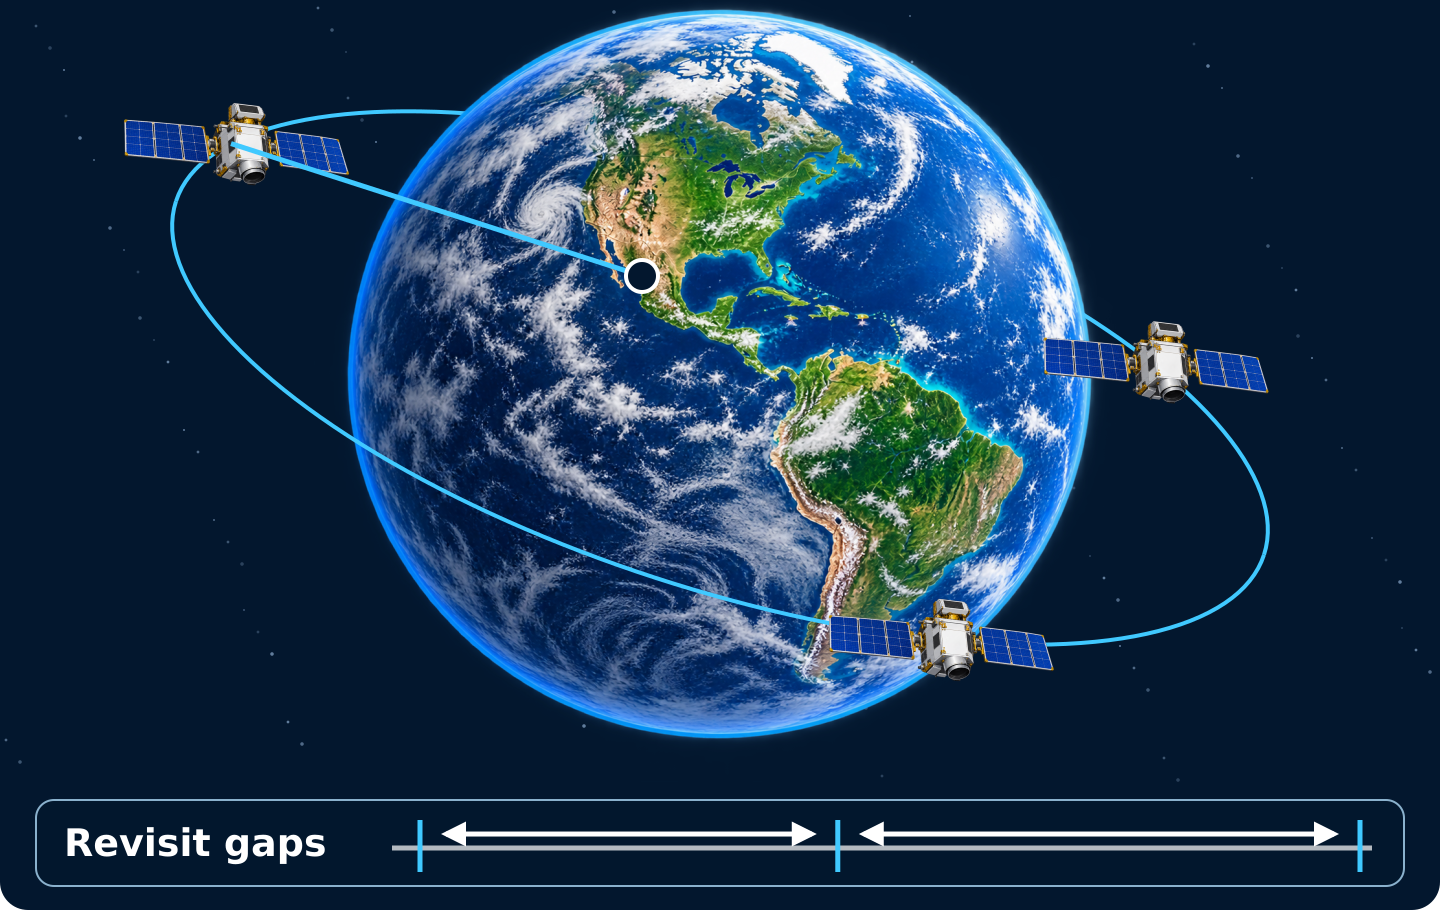
\includegraphics[width=0.94\linewidth]{tour-revisit.png}\\[0.08em]
      {\scriptsize\bfseries Design constellations}\\[0.05em]
      \parbox[t][1.7em][t]{\linewidth}{\centering\tiny Revisit}
    \column{0.245\textwidth}\centering
      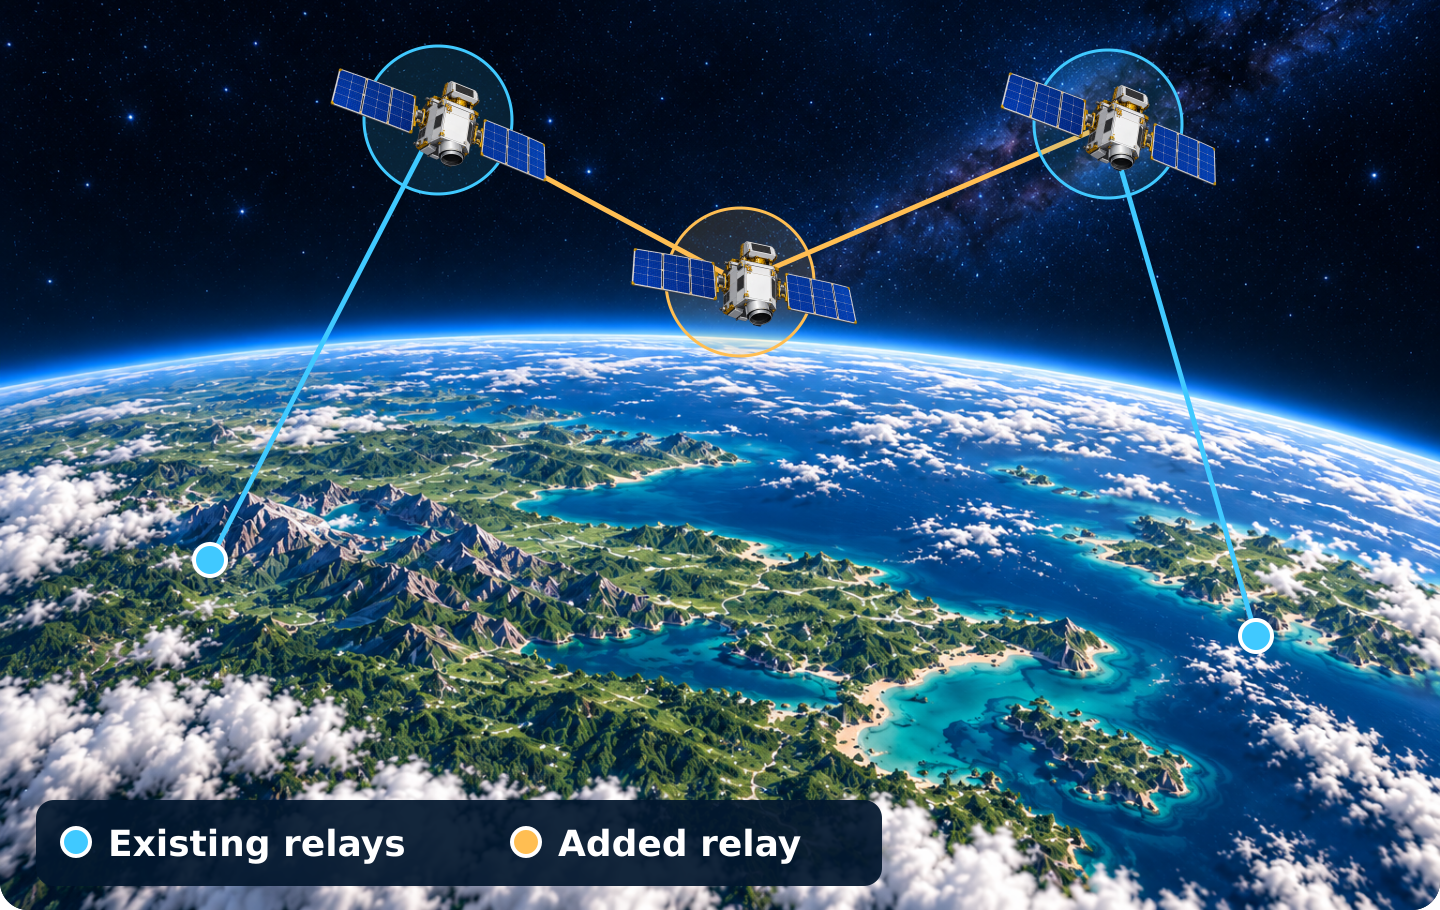
\includegraphics[width=0.94\linewidth]{tour-relay.png}\\[0.08em]
      {\scriptsize\bfseries Augment relay networks}\\[0.05em]
      \parbox[t][1.7em][t]{\linewidth}{\centering\tiny Relay}
  \end{columns}
  \vspace{0.2em}
  {\footnotesize
  \setlength{\tabcolsep}{4pt}
  \begin{tabularx}{\textwidth}{@{}l X r@{}}
    \toprule
    \textbf{Decision} & \textbf{Families and submission} & \textbf{Scale} \\
    \midrule
    Observe Earth & AEOSSP, SPOT-5, Regional, Stereo & 8 photos--18.3k cells \\
    Allocate contacts & SatNet: antenna-track assignment & 257--333 requests; 7\,d \\
    Design constellations & Revisit: constellation + schedule & 24--32 targets; 48\,h \\
    Augment relay networks & Relay: added satellites + link plan & 6--10 sats; 4--8 demands \\
    \bottomrule
  \end{tabularx}}
  \par\vspace{0.3em}
  \srcnote{Orbits from real CelesTrak TLE snapshots; targets from public city/site/region libraries; SatNet \& SPOT-5 normalized from published benchmarks.}
\end{frame}

% ================= 6. Evaluation contract =================
\begin{frame}{Validity first, then mission value}
  \begin{columns}[T]
    \column{0.50\textwidth}
      \begin{beamercolorbox}[rounded=true,sep=0.6em]{block body}
        \begin{minipage}[t][5.85cm][c]{\dimexpr\linewidth-1.2em\relax}
        \cardtitle{1. Validity, checked first by re-simulation}
        {\small\raggedright The artifact arrives before timeout and parses into the family's decision schema. The verifier recomputes time windows, geometry, and resource budgets over the horizon.\par}
        \vspace{0.7em}
        \cardtitle{2. Performance, computed only if valid}
        {\small\raggedright Family-native metrics grade coverage, service, revisit gap, or profit, normalized to a 0--100 scale. Missing or invalid plans receive zero.\par}
        \end{minipage}
      \end{beamercolorbox}
    \column{0.50\textwidth}
      \begin{beamercolorbox}[rounded=true,sep=0.7em]{block body}
        \begin{minipage}[t][5.85cm][c]{\dimexpr\linewidth-1.4em\relax}
        \cardtitle{Worked example: AEOSSP case 1}
        {\footnotesize\color{abgray} Claude Code + Claude Opus 4.6, one of five held-out cases\par}
        \vspace{0.3em}
        {\scriptsize
        \begin{tabular}{@{}l r@{}}
        tasks completed & 1,415 / 1,947 \\
        weight recovered & 68.5\% \\
        mean turnaround & 1,071 / 43,200\,s \\
        energy used & 18.6 / 31.0\,kWh \\
        \midrule
        \textbf{normalized score} & \textbf{70.87} \\
        \end{tabular}\par}
        \vspace{0.4em}
        {\color{abgray!40}\rule{\linewidth}{0.4pt}}
        \vspace{0.4em}
        {\footnotesize\raggedright A fifth case parsed as an empty schedule and scored \textcolor{abred}{\textbf{0}}, pulling the five-case mean down to \textbf{58.45}.\par}
        \end{minipage}
      \end{beamercolorbox}
  \end{columns}
  \vspace{0.2em}
  \centering
  {\footnotesize\color{abgray} Every plan is judged first on validity, then on value.}
\end{frame}

% ================= 7. Setup =================
\begin{frame}{Five agent systems, one controlled protocol}
  \begin{columns}[T]
    \column{0.52\textwidth}
      \cardtitle{Evaluated systems}
      {\small
      \setlength{\tabcolsep}{4pt}
      \begin{tabularx}{\linewidth}{@{}l l@{}}
        \toprule
        \textbf{Harness} & \textbf{Model} \\
        \midrule
        Claude Code & Claude Opus 4.6 \\
        Codex CLI & GPT-5.4 \\
        Kimi CLI & Kimi K2.6 \\
        OpenCode & MiniMax M2.7 \\
        OpenCode & DeepSeek V4 Pro \\
        \bottomrule
      \end{tabularx}}
      \vspace{0.4em}

      {\scriptsize\color{abgray} A \emph{system} = model + harness + workspace; the same model in a different harness is a different system.}
    \column{0.48\textwidth}
      \hspace*{0.8em}\cardtitle{Protocol}
      \begin{itemize}\setlength{\itemsep}{0.35em}
        \item \textbf{35 held-out cases}, 5 per family
        \item \textbf{2\,h wall-clock}, 8 CPU cores, 32\,GB RAM
        \item Scientific + astrodynamics + OR libraries preinstalled
        \item Artifact scored \textbf{after the run} by the official verifier; no human repair
      \end{itemize}
  \end{columns}
\end{frame}

\section{Results}

% ================= 8. Main results =================
\begin{frame}{Agents plan for real: promising, but highly uneven}
  \centering
  \newlength{\resw}\setlength{\resw}{0.72\textwidth}
  \newlength{\resh}\setlength{\resh}{\dimexpr\resw*1266/2312\relax}
  \begin{tikzpicture}[x=\resw,y=\resh]
    \node[anchor=south west,inner sep=0] (img) at (0,0) {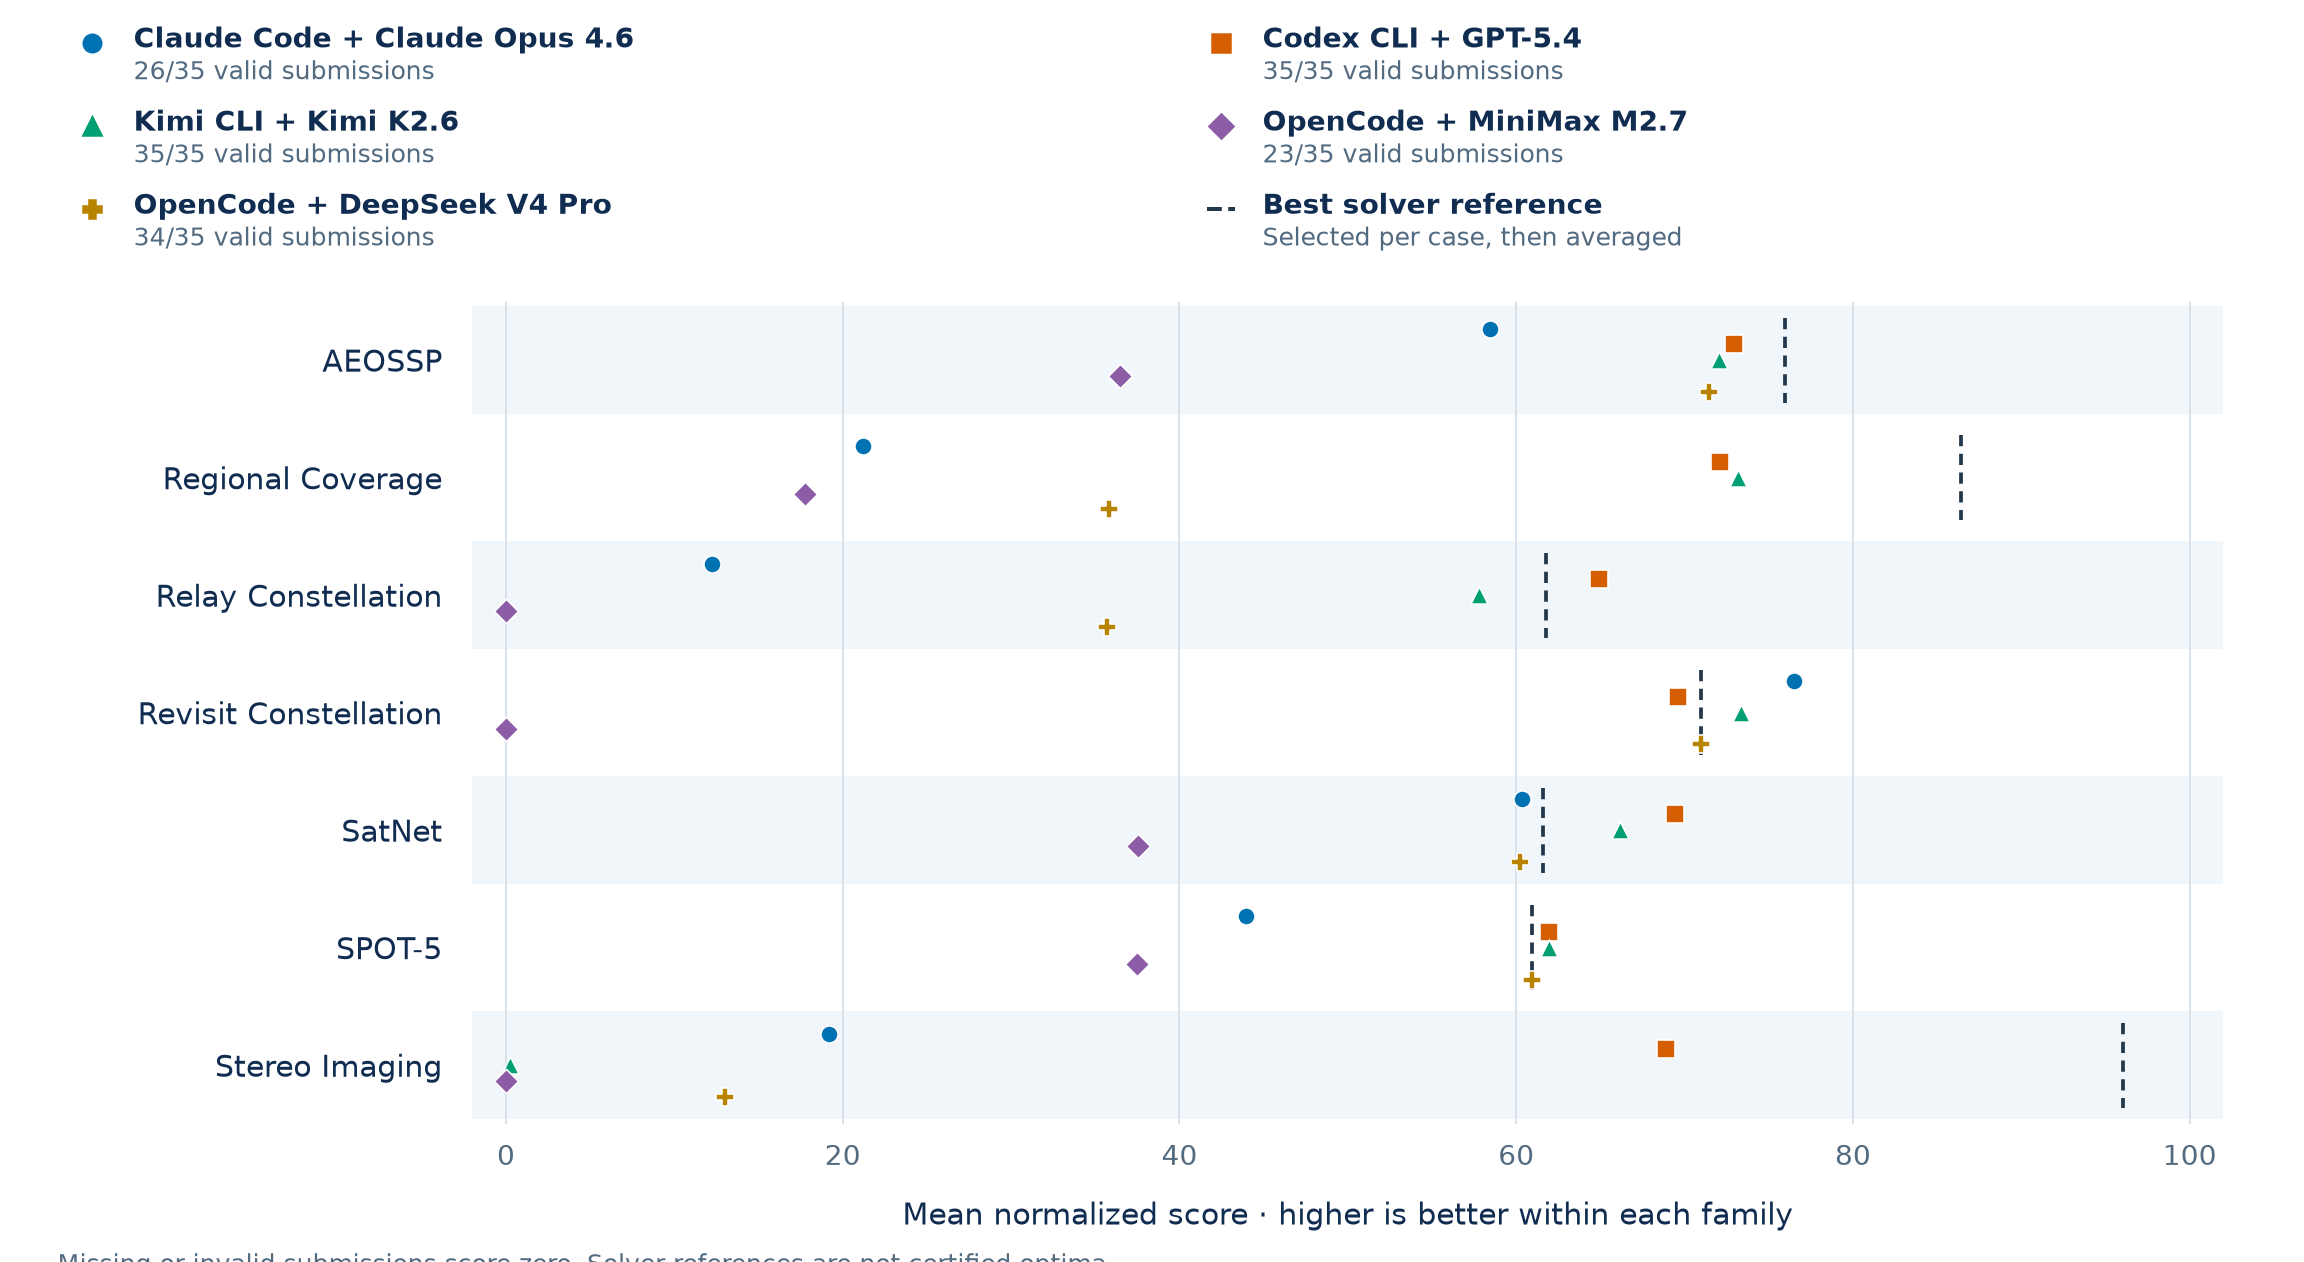
\includegraphics[width=\resw]{initial-results-plot.png}};
    \node[anchor=west,fill=white,draw=abgray!50,rounded corners=2pt,inner sep=3.5pt,font=\scriptsize,align=left] at (1.02,0.24) {\textcolor{abcyan}{SatNet} $+7.9$\\[0.15em] \textcolor{abred}{Stereo} $-27$};
  \end{tikzpicture}
  \par\vspace{0.15em}
  {\scriptsize 35/35 valid (Codex, Kimi); best agent row beats solver on 4/7 families; two families lag by 13--27 points.}
\end{frame}

% ================= 9. Reading the results =================
\begin{frame}{Validity is achievable; value is the frontier}
  \begin{columns}[T]
    \column{0.31\textwidth}
      \stat{35/35}{verifier-valid submissions\\(Codex + GPT-5.4; Kimi + K2.6)}
      \vspace{0.5em}
      \parbox[t][2.4em][t]{\linewidth}{\small Yet \textbf{valid $\neq$ valuable}: even fully valid systems leave large score gaps.}
    \column{0.31\textwidth}
      \stat{4/7}{families where the best agent row \textbf{beats} solver references}
      \vspace{0.5em}
      \parbox[t][2.4em][t]{\linewidth}{\small SPOT-5 $+1.0$ \,\textperiodcentered\, Relay $+3.1$ \,\textperiodcentered\, Revisit $+5.5$ \,\textperiodcentered\, SatNet $+7.9$; AEOSSP within $-3.0$.}
    \column{0.31\textwidth}
      \stat{13--27\vphantom{/}}{point gaps remain on Regional Coverage and Stereo Imaging}
      \vspace{0.5em}
      \parbox[t][2.4em][t]{\linewidth}{\small Design-heavy tasks stay hard, and \textbf{leaders differ across systems}.}
  \end{columns}
  \vspace{0.9em}
  \centering
  {\scriptsize Agent $-$ solver reference (points; positive means the agent is ahead)}\par\vspace{0.1em}
  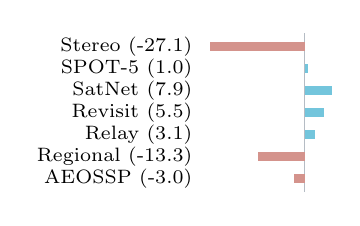
\begin{tikzpicture}[x=0.21cm,y=0.28cm,font=\scriptsize]
    \draw[abgray!45] (0,-0.6) -- (0,6.6);
    \foreach \y/\name/\val in {%
      0/AEOSSP/-3.0, 1/Regional/-13.3, 2/Relay/3.1,
      3/Revisit/5.5, 4/SatNet/7.9, 5/SPOT-5/1.0, 6/Stereo/-27.1} {
      \pgfmathsetmacro{\x}{\val*0.21}
      \node[anchor=east] at (-6.2,\y) {\name\ (\val)};
      \pgfmathparse{\val<0 ? 1 : 0}
      \ifnum\pgfmathresult=1
        \fill[abred!55] (\x,\y-0.20) rectangle (0,\y+0.20);
      \else
        \fill[abcyan!55] (0,\y-0.20) rectangle (\x,\y+0.20);
      \fi
    }
  \end{tikzpicture}
\end{frame}

\section{Analysis}

% ================= 10. Failure modes =================
\begin{frame}{Where runs fail: two distinct layers}
  \begin{columns}[T]
    \column{0.48\textwidth}
      \begin{beamercolorbox}[rounded=true,sep=0.7em]{block body}
        \begin{minipage}[t][4.5cm][t]{\dimexpr\linewidth-1.4em\relax}
        \cardtitle{1. Task-formulation failures}
        {\small The system misreads the task contract and builds a \textbf{self-imposed task}: an inferred schema and a hallucinated objective, missing physical constraints or the required artifact format.\\[0.2em]
        \emph{Stereo Imaging:} valid observations never form eligible products; local validation accepts what the official verifier rejects.}
        \end{minipage}
      \end{beamercolorbox}
    \column{0.48\textwidth}
      \begin{beamercolorbox}[rounded=true,sep=0.7em]{block body}
        \begin{minipage}[t][4.5cm][t]{\dimexpr\linewidth-1.4em\relax}
        \cardtitle{2. Solution-construction failures}
        {\small The task contract is understood, but the run cannot reliably \textbf{build, improve, and preserve} a high-value executable plan. Failures appear as weak search, brittle code, late verifier use, or silent goal drift.\\[0.2em]
        \emph{Relay:} valid-but-zero-value submissions accepted as done; agent-written simulators trusted after verifier disagreement.}
        \end{minipage}
      \end{beamercolorbox}
  \end{columns}
  \vspace{0.9em}
  \begin{columns}[T]
    \column{0.31\textwidth}\stat[abred]{12.6\%}{of 175 runs end\\with an invalid plan}
    \column{0.31\textwidth}\stat[abred]{9.1\%}{submit a valid artifact\\scoring zero}
    \column{0.31\textwidth}\stat[abred]{22.3\%}{commit an artifact before\\reading the task contract}
  \end{columns}
\end{frame}

% ================= 11. Success mechanisms =================
\begin{frame}{What strong runs do differently}
  \begin{columns}[c]
    \column{0.50\textwidth}
      \begin{itemize}\setlength{\itemsep}{1.1em}
        \item \textbf{Implementation calibration.} Agents write propagation and scheduling code, then repair it against \textbf{verifier disagreement} before trusting it.
        \item \textbf{Case-adaptive search with incumbent preservation.} Strong runs infer the \emph{case-specific} bottleneck and always keep the best verified plan.
      \end{itemize}
    \column{0.50\textwidth}
      \cardtitle{Mean verifier calls per case}
      {\scriptsize
      \setlength{\tabcolsep}{2.5pt}
      \begin{tabular}{lccccc}
        \toprule
        System & Rev. & Ste. & Sat. & Reg. & Rel. \\
        \midrule
        Claude & 13.6 & \cellcolor{abgray!18}20.2\textsuperscript{2} & \cellcolor{abgray!18}19.0\textsuperscript{1} & \cellcolor{abgray!18}0.0\textsuperscript{5} & \cellcolor{abgray!18}1.0\textsuperscript{4} \\
        Codex & 5.8 & 8.8 & 6.0 & 8.2 & 6.4 \\
        Kimi & 9.2 & 10.4 & 16.0 & 11.6 & 8.8 \\
        OC+MM & \cellcolor{abgray!18}3.0\textsuperscript{4} & \cellcolor{abgray!18}18.0\textsuperscript{3} & 19.4 & \cellcolor{abgray!18}25.8\textsuperscript{1} & 19.4 \\
        OC+DS & 6.0 & 47.2 & 10.0 & 18.2 & 12.4 \\
        \bottomrule
      \end{tabular}}
      \par\vspace{0.5em}
      \srcnote{Gray: at least one zero-call case (superscript = count); these runs never calibrated against the official model.}
  \end{columns}
  \vspace{1.0em}
  \centering
  {\small Solvers are systematic, but their adaptation policy is fixed before the run.\\[0.3em]
  Strong agent runs \textbf{synthesize the search policy during the run}.}
\end{frame}

% ================= 12. Trace evidence =================
\begin{frame}{Three traces, three mechanisms}
  \begin{columns}[T]
    \column{0.32\textwidth}
      \begin{beamercolorbox}[rounded=true,sep=0.65em]{block body}
        \begin{minipage}[t][2.8cm][t]{\dimexpr\linewidth-1.4em\relax}
        \cardtitle[abred]{Private world}
        \vspace{0.3em}
        \stat[abred]{0}{official score}
        \vspace{0.35em}
        {\scriptsize\raggedright Agent-side check passed; the official verifier rejected it.\par}
        \end{minipage}
      \end{beamercolorbox}
    \column{0.32\textwidth}
      \begin{beamercolorbox}[rounded=true,sep=0.65em]{block body}
        \begin{minipage}[t][2.8cm][t]{\dimexpr\linewidth-1.4em\relax}
        \cardtitle[abgold]{Calibration}
        \vspace{0.3em}
        \stat[abgold]{+0.041$^\circ$}{beyond the 30$^\circ$ off-nadir limit}
        \vspace{0.35em}
        {\scriptsize\raggedright Propagation and frame handling are repaired until they match the benchmark.\par}
        \end{minipage}
      \end{beamercolorbox}
    \column{0.32\textwidth}
      \begin{beamercolorbox}[rounded=true,sep=0.65em]{block body}
        \begin{minipage}[t][2.8cm][t]{\dimexpr\linewidth-1.4em\relax}
        \cardtitle[abcyan]{Adaptive search}
        \vspace{0.3em}
        \stat[abcyan]{55}{targeted demand samples}
        \vspace{0.35em}
        {\scriptsize\raggedright An empty but valid baseline is kept while search targets the bottleneck.\par}
        \end{minipage}
      \end{beamercolorbox}
  \end{columns}
\end{frame}


% ================= 13. Ablations =================
\begin{frame}{Workspace support aids planning conditionally}
  \begin{columns}[T]
    \column{0.42\textwidth}
      \centering
      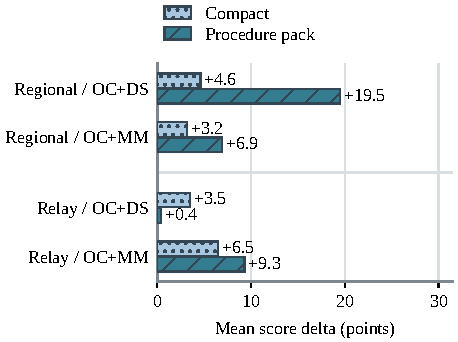
\includegraphics[width=0.98\linewidth]{ablation_procedure.pdf}\\[-0.2em]
      {\small\bfseries (A) Procedure injection}
    \column{0.42\textwidth}
      \centering
      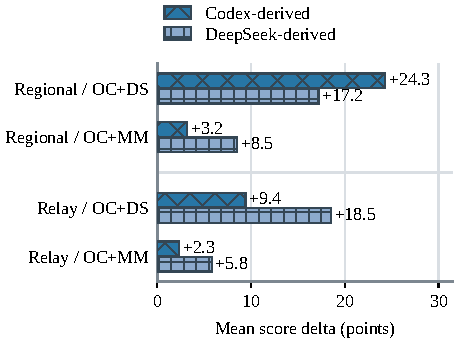
\includegraphics[width=0.98\linewidth]{ablation_memory.pdf}\\[-0.2em]
      {\small\bfseries (B) Memory accumulation}
  \end{columns}
  \vspace{0.4em}
  \centering
  \small Deltas vs.\ no-support baseline (OpenCode systems). Support helps \textbf{when it supplies the missing formulation, calibration, or search discipline}.
\end{frame}

\section{Takeaways}

% ================= 14. Takeaways =================
\begin{frame}{Takeaways}
  \vspace{0.1em}
  {\large\bfseries\color{abnavy} Agentic space mission planning shows nontrivial ability and clear brittleness.}\par
  \vspace{0.4em}
  \begin{columns}[c]
    \column{0.62\textwidth}
      {\small
      \begin{itemize}\setlength{\itemsep}{0.45em}
        \item \textbf{Executable} space mission planning: 7 families, 116 cases, external feasibility checks, graded mission value.
        \item Best agent rows \textbf{beat solver references on 4 of 7 families}, yet capability remains \textbf{uneven and system-dependent}.
        \item Success tracks \textbf{verifier-calibrated implementations} and \textbf{case-adaptive search}; failures separate into \textbf{task-contract misformulation} and \textbf{weak solution construction}.
      \end{itemize}}
    \column{0.36\textwidth}
      \centering
      \begin{columns}[T]
        \column{0.48\linewidth}\centering
          
\includegraphics[width=0.75\linewidth]{qr_github.png}\\[0.05em]
          \parbox[t][2.0em][t]{\linewidth}{\centering\tiny Code \& cases\\ GitHub}
        \column{0.48\linewidth}\centering
          
\includegraphics[width=0.75\linewidth]{qr_hf.png}\\[0.05em]
          \parbox[t][2.0em][t]{\linewidth}{\centering\tiny Taskset\\ Hugging Face}
      \end{columns}
      \vspace{0.2em}
      \begin{columns}[T]
        \column{0.48\linewidth}\centering
          
\includegraphics[width=0.75\linewidth]{qr_arxiv.png}\\[0.05em]
          \parbox[t][2.0em][t]{\linewidth}{\centering\tiny Paper\\ arXiv 2601.11354}
        \column{0.48\linewidth}\centering
          
\includegraphics[width=0.75\linewidth]{qr_zenodo.png}\\[0.05em]
          \parbox[t][2.0em][t]{\linewidth}{\centering\tiny Run archive\\ Zenodo}
      \end{columns}
  \end{columns}
\end{frame}

\end{document}
